\begin{changemargin}{-3.6cm}{0cm}
	
\parbox{.4in}{
    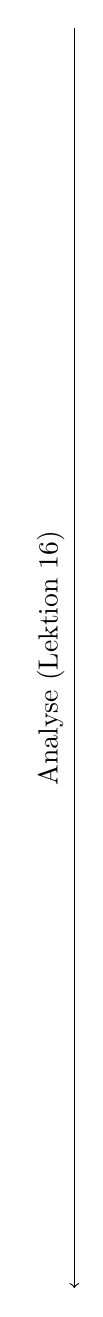
\begin{tikzpicture}
	\draw[<-] (0,0) -- node[rotate=90,above]{Analyse (Lektion 16)} (0,16);
    \end{tikzpicture}
}
\parbox{3in}{
    \begin{itemize}
	\item Karateristiske ligninger
	\item Exitationsligninger
	\item outputligninger
    \end{itemize}
    ---
    \begin{itemize}
	\item List alle kombinationer af $Q_n,\ldots,Q_0$
	\item Udfyld $Q^*$ Vha. ligningerne
	\item Udfyld output cha. ligningerne
    \end{itemize}
    ---
    \begin{itemize}
	\item Giv hver tilstand et navn
	\item Udfyld $T^*$
    \end{itemize}
    ---
    \begin{itemize}
	\item Tegn en ``Bolle'' for hver tilstand
	\item Tiføj pile og \colorul{red}{outputs}
    \end{itemize}
    ---
    \begin{itemize}
	\item Lav en række for $T$ vha. pilediagrammet
	\item Udfyld outputs
    \end{itemize}
}
\parbox{1.2in}{
    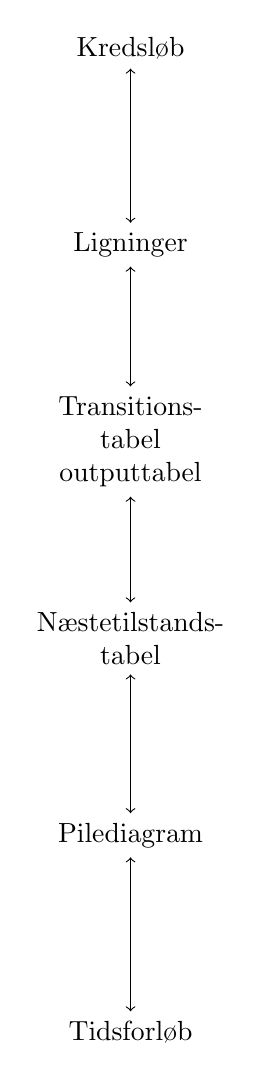
\begin{tikzpicture}
	\node at (0,0) (A) {Tidsforløb};
	\node at (0,2.5) (B) {Pilediagram};
	\node[align=center] at (0,5) (C) {Næstetilstands-\\tabel};
	\node[align=center] at (0,7.5) (D) {Transitions-\\tabel\\outputtabel};
	\node at (0,10) (E) {Ligninger};
	\node at (0,12.5) (F) {Kredsløb};
	\draw[<->] (A) -- (B);
	\draw[<->] (B) -- (C);
	\draw[<->] (C) -- (D);
	\draw[<->] (D) -- (E);
	\draw[<->] (E) -- (F);
    \end{tikzpicture}
}
\parbox{3in}{
    \begin{itemize}
	\item Tegn alle D-flip-Flops
	\item Husk synkron clk
	\item Tegn exitationslogik
	\item tegn outputlogik
	\item Selvkorrigerende
    \end{itemize}
    ---
    \begin{itemize}
	\item Bestem all $Q^*=D$ og outputs (evt.\ vha.\ k-kort) ``simple'' logiske kredsløb med $Q_n,\ldots,Q_0$ og brugerinputs som input. Nyt k-kort for \emph{hver} $Q^*=D$ og output.
    \end{itemize}
    ---
    \begin{itemize}
	\item Bestem antal D-flip-Flops
	\item Tildel en bitkombination til hver tilstand

	    Lad $Q^*$ være don't care for ubrugte Tilstandsmaskiner
	\item Tilføj outputs
    \end{itemize}
    ---
    \begin{itemize}
	\item Lav $T$ og $T^*$ søjlr vha.\ pilediagrammet
    \end{itemize}
    ---
    \begin{itemize}
	\item Bestem antallet af tilstande, og tegn pilediagrammet (se på sekvenslængden)
    \end{itemize}
}
\nolinebreak
\parbox{.5cm}{\ }
\nolinebreak
\parbox{.4in}{
    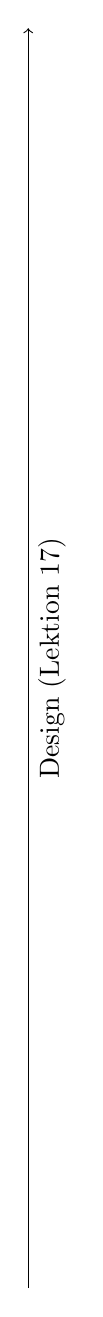
\begin{tikzpicture}
	\draw[->] (0,0) -- node[rotate=90,below]{Design (Lektion 17)} (0,16);
    \end{tikzpicture}
}

\end{changemargin}
